\chapter{Optimal Control and Non-Linear Optimization Basics\label{chapter:optimization}}

\ifpdf
    \graphicspath{{ChapterOptimizationIntroduction/figures/Raster/}{ChapterOptimizationIntroduction/figures/PDF/}{ChapterOptimizationIntroduction/figures/}}
\else
    \graphicspath{{ChapterOptimizationIntroduction/figures/Vector/}{ChapterOptimizationIntroduction/figures/}}
\fi

In previous chapters, we investigated the tools for modeling a floating base system that establishes a set of contacts with the environment. This chapter introduces the basics and terminology of \emph{non-linear programming} and \emph{optimal control}. We then take advantage of the technique presented here to design the controllers analyzed in Part~\ref{part:wbc} and Part~\ref{part:simplified}.
Non-linear programming is the mathematical process of finding a set of variables such that a non-linear function is minimized (or maximized). Once the theory of \emph{non-linear programming} is introduced, we apply it to the resolution of the \emph{optimal control} problems. 
The \emph{optimal control theory} is a branch of control theory that aims at finding a control for a dynamic system over a period of time such that an objective function is optimized.
\par
The chapter will take an \emph{utilitaristic} approach to describe such frameworks, to this concern we decided to avoid focusing on the rigorous proofs. The reader who wants a more rigorous understanding of non-linear optimization theory should consult the extensive literature. Here, it is worth mentioning \citep{Boyd2004ConvexOptimization,Chachuat2007NonlinearPractice,diehl2009efficient} from which parts of this chapter took inspiration. On the other hand, complete and rigorous manuscripts on optimal control are \citep{Boyd2004ConvexOptimization,bemporad2002hybrid,Qin2000AnApplications,Biral2016NotesProblems,Allgower1999NonlinearOverview}.
\par
The chapter is organized as follows.
Sections~\ref{sec:convex_set} and~\ref{sec:convex_function} give an overview of convex sets and convex functions, respectively. Section~\ref{sec:optionization_problem} introduces the optimization problem. Section~\ref{sec:qp} presents the Quadratic Programming problem as a special case of the optimization problem. The Quadratic Programming problem will be extensively exploited in the design of the whole-body controllers presented in Part~\ref{part:wbc}.  Section~\ref{sec:optimal_control} and \ref{sec:mpc} introduce some of the basics of Optimal Control and Model Predictive Control. The content of Section~\ref{sec:mpc} will be crucial to fully comprehend the design of the controllers detailed in Part~\ref{part:simplified}.


\section{Convex set\label{sec:convex_set}}

\subsection{Affine and convex sets\label{sec:affine_convex_sets}}
Given two points, $x_1, x_2$ in a set $\mathbb{R}^n$ such that $x_1 \ne x_2$, we define $y\in\mathbb{R}^n$ the \emph{line} passing through $x_1$ and $x_2$ as
\begin{equation}
    y = \theta x_1 + ( 1-\theta) x_2,
\end{equation}
where $\theta \in \mathbb{R}$. When $\theta = 1$, $y$ coincides with $x_1$, while if $\theta = 0$, $y = x_2$.
A set $C$ is affine if given two distinct points in $C$ the line connecting them belongs to $C$, i.e., for any $x_1, x_2 \in C$, and $theta = [0,1]$ then $\theta x_1 + ( 1-\theta) x_2 \in C$. Given a set of points $x_1, x_2, \dots, x_n$, we define the \emph{affine combination of} $x_1, x_2, \dots, x_n$, $\theta_1 x_1 +  \theta_2 x_2 + \dots + \theta_n x_n$ where  $\theta_1+ \theta_2+ \dots +  \theta_n = 1$ and $\theta_i \ge 0$ for $i = 1, \dots, n$.

\subsubsection{Convex sets}
A set $C$ is said to be \emph{convex} if the line segment between two points in $C$ belongs to $C$. More formally, given any $x_1, x_2 \in C$ and any $\theta$ such that $0 \le \theta \le 1$ $\theta x_1 + ( 1-\theta) x_2 \in C$.
To give the reader a better understanding, a set is convex if every point in the set can be connected with an unobstructed straight path between them. Figure~\ref{fig:convex_set} illustrates an example of a convex set, while Figure~\ref{fig:nonconvex_set} presents an example of a nonconvex set.
\par
Given $n$ points, $x_1, x_2, \dots, x_n$, and $\theta_1, \theta_2, \dots, \theta_n \in \mathbb{R}$ such that $\theta_1+ \theta_2+ \dots +  \theta_n = 1$ and $\theta_i \ge 0$ for $i = 1, \dots, n$, the \emph{convex combination} of $x_1, x_2, \dots, x_n$ is given by $\theta_1 x_1 +  \theta_2 x_2 + \dots + \theta_n x_n$.
\par
The \emph{convex hull} of a set $C$, denoted with $\conv C$, is the set of all the convex combinations of the points in $C$ and it is written as:
\begin{equation}
    \conv C = \left\{ \theta_1 x_1 +  \theta_2 x_2 + \dots + \theta_n x_n | x_i \in C, \theta_i \ge 0, i=1,\dots, n,\; \sum_{i = 1}^{n} \theta_i = 1 \right\}.
\end{equation}
Here we underline that the convex hull of $C$ is a convex set 
\begin{figure}[t]
\centering
    \begin{subfigure}[b]{0.48\textwidth}
        \centering
        \includegraphics{chapter_optimization_introduction/figures/convex_set.tikz}
        \caption{Convex set.}
        \label{fig:convex_set}
    \end{subfigure}
    \hfill
    \begin{subfigure}[b]{0.48\textwidth}
        \centering
        \includegraphics{chapter_optimization_introduction/figures/nonconvex_set.tikz}
        \caption{Nonconvex set.}
        \label{fig:nonconvex_set}
    \end{subfigure}
	\caption[Examples of convex and nonconvex sets]{Examples of convex and nonconvex sets. (a) The oval shape is a convex set (b) The \emph{'s'} shaped set is not convex, since the red line segment between $x_1$ and $x_2$ in not fully contained in the set.}
	\label{fig:convex_nonconvex_sets}
\end{figure}
\subsubsection{Convex cones}
A set $C$ is \emph{cone} if for every point $x \in C$ and a real positive parameter $\theta \ge 0$, $\theta x \in C$. Given a cone $C$, if it is convex, we say that $C$ is a \emph{convex cone}, thus for any $x_1, x_2 \in C$ and $\theta_1, \theta_2 \ge 0$ the affine combination of $x_1, x_2$ belongs to $C$, i.e  $\theta_1 x_1 + \theta_2 x_2 \in C$.
\par
Given $n$ points $x_1, x_2, \dots, x_n$, and $\theta_1, \theta_2, \dots, \theta_n \in \mathbb{R}$ such that $\theta_i \ge 0$ for $i = 1, \dots, n$, the \emph{conic combination} of $x_1, x_2, \dots, x_n$ is given by $\theta_1 x_1 +  \theta_2 x_2 + \dots + \theta_n x_n$. Here, it is worth recalling that if $x_i$ is in a convex cone $C$, then every conic combination of $x_i$ belongs in $C$
The \emph{conic hull} of a set $C$, denoted by $\conic C$, is the set of all the conic combinations of the points in $C$ and it writes as:
\begin{equation}
    \conic C = \left\{ \theta_1 x_1 +  \theta_2 x_2 + \dots + \theta_n x_n | x_i \in C, \theta_i \ge 0, i=1,\dots, n\right\}.
\end{equation}

\subsection{Convex set examples\label{sec:convex_set_example}}
In this section, we recall some important examples of convex sets that we will encounter throughout the rest of the manuscript. We first introduce the hyperplanes, halfspaces and then second-order cones, also known as Lorentz cones. We conclude the section by presenting the polyhedra and the associated \emph{Minkowski-Weyl} theorem.

\subsubsection{Hyperplanes and halfspaces}
Given a set $H$, we say that $H$ is an \emph{Hyperplane} if it can be represented in the form 
\begin{equation}
    \label{eq:hyperplane}
    H = \{ x \in \mathbb{R}^n | a^\top x = b \},
\end{equation}
where $a \in \mathbb{R}^n$ and $b$ is a real number. The hyperplane representation can be seen as the set of points with a constant scalar product with a vector $a$. Similarly, $a$ can be seen as the \emph{normal vector} of the plane. $b$ is the offset of the plane from the origin.  Given any point $x_0$ in the hyperplane, Equation~\eqref{eq:hyperplane} can be rewritten as $\{ x \in \mathbb{R}^n | a^\top  ( x - x_0) = 0 \}$
\par
A hyperplane splits the space into two \emph{halfspaces}. We define a \emph{closed} halfspace as the convex set $\{ x \in \mathbb{R}^n | a^\top   x \le  b \}$. We note that the halspace $a^\top   x \ge  b$ is the halfspace extending in the direction of the vector $a$, while $a^\top   x \le  b$ contains $-a$ -- see Figure~\ref{fig:hyperplane}.

\subsubsection{Second order cone}
Given a vector $x \in \mathbb{R}^n$,  the Euclidean norm in $\mathbb{R}^n$ $\| \;\; \|$ and a positive scalar $t$, we define the \emph{second order cone} as
\begin{IEEEeqnarray}{ll}
\phantomsection \label{eq:lorentz_cone} \IEEEyesnumber \IEEEyessubnumber*    \mathcal{Q}^{n+1} &=  \left\{ \left. \begin{bmatrix}x \\ t\end{bmatrix} \in \mathbb{R}^{n+1} \; \right| \; \| x \| \le t \right\}  \\
&=\left\{ \left. \begin{bmatrix}x \\ t\end{bmatrix} \in \mathbb{R}^{n+1} \; \right| \; \begin{bmatrix}x \\ t\end{bmatrix} ^\top 
    \begin{bmatrix}
    I_n & 0_{n \times 1} \\
    0_{1\times n }& -1
    \end{bmatrix} 
    \begin{bmatrix}x \\ t\end{bmatrix} \le 0, t\ge 0
    \right\}.
\end{IEEEeqnarray}
The second-order cone, often named \emph{Lorentz cone}, is a convex cone. 
\par
We notice that, in the context of rigid contact modeling, the friction cone (Equation~\eqref{eq:friction_cone}) is a Lorentz cone. Indeed, given the point in contact with the environment and a contact force $f\in\mathbb{R}^3$, we say that $f$ belongs to the friction cone if and only if 
\begin{equation}
    \label{eq:friction_cone_convex}
    \sqrt{f_1 ^2 + f_2^2} \le \mu f_3,
\end{equation}
where $\mu$ is the static friction coefficient, or in other words, 
\begin{equation}
    \label{eq:friction_cone_convex_set}
    f \in \left\{f\in\mathbb{R}^3 \; | \;\sqrt{f_1 ^2 + f_2^2} \le \mu f_3\right\}.
\end{equation}
Setting $\mu f_3 = t$ and $x^\top = \begin{bmatrix}
f_1 & f_2 \end{bmatrix}$, Equation~\eqref{eq:friction_cone_convex_set} is equivalent to~\eqref{eq:lorentz_cone}. Thus, we can conclude that the friction cone is an example of the Lorenz cone.
\begin{figure}[t]
\centering
    \begin{subfigure}[b]{0.35\textwidth}
        \centering
        \includegraphics{chapter_optimization_introduction/figures/polyhedron.tikz}
        \caption{}
        \label{fig:polyhedron}
    \end{subfigure}
     \begin{subfigure}[b]{0.15\textwidth}
        \centering
        \includegraphics{chapter_optimization_introduction/figures/cone.tikz}
        \caption{}
        \label{fig:cone}
    \end{subfigure}    
    \hfill
    \begin{subfigure}[b]{0.35\textwidth}
        \centering
        \includegraphics{chapter_optimization_introduction/figures/polytope.tikz}
        \caption{}
        \label{fig:polytope}
    \end{subfigure}
	\caption[Examples of polyhedra]{Examples of polyherda. The orange circle denotes the vertices of the polyhedra, while the green arrows the rays. (a) The $\mathcal{V}$\emph{-rep} of a generic polyhedron is composed by vertices and rays. (b) A polyhedral cone is described by rays. (c) The $\mathcal{V}$\emph{-rep} of a polytope consist in vertices only}
	\label{fig:polyhedron-polytope}
\end{figure}
\subsubsection{Polyhedra \label{sec:polyhedra}}
We define a \emph{polyhedron}, denoted as $\mathcal{P}$, as the solution set of a finite number of linear inequalities and equalities such that:
\begin{equation}
    \label{eq:polyhedron_def}
    \mathcal{P} = \{ x \; | \; a_i ^\top x \le b_i, \, i = 1, \dots, m, \,  c_j ^\top x = d_j \, j = 1,\dots,n\}.
\end{equation}
Often the equalities $c_j ^\top x = d_j$ are not considered in the polyhedron formulation. In fact, equality can always be replaced with two inequalities, for instance $c_j ^\top x = d_j$ is equivalent to $c_j ^\top x \le d_j$ and $-c_j ^\top x \le -d_j$. Considering this, in the following we will remove the equality terms from the polyhedron definition. Thus we write~\eqref{eq:polyhedron_def} as
\begin{equation}
    \label{eq:polyhedron_def_ineq}
    \mathcal{P} = \{ x \; | \; a_i ^\top x \le b_i, \, i = 1, \dots, k \},
\end{equation}
where $k = m + 2 n$.
It is worth noting that a polyhedron can be seen as the intersection of finite halfspaces and hyperplanes. Hereafter, we call a bounded polyhedron \emph{polytope}.
Figure~\ref{fig:polyhedron} illustrates an example of a polyhedron, while Figure~\ref{fig:polytope} a polytope.
Equation~\eqref{eq:polyhedron_def_ineq} is often written in a more compact from as
\begin{equation}
    \label{eq:polyhedron_def_compact}
    \mathcal{P} = \{ x \; | \; A x \preceq b \},
\end{equation}
where $b = \begin{bmatrix}
b_1& \hdots & b_m
\end{bmatrix}^\top$. While $A$ is given by
\begin{equation}
    A = \begin{bmatrix}
        a_1^\top \\
        \vdots \\
        a_m^\top
    \end{bmatrix}. 
\end{equation}
\begin{figure}[t]
\centering
    \begin{subfigure}[b]{0.48\textwidth}
        \centering
        \includegraphics{chapter_optimization_introduction/figures/hyperplane.tikz}
        \caption{Geometric representation of a hyperplane.}
        \label{fig:hyperplane}
    \end{subfigure}
    \hfill
    \begin{subfigure}[b]{0.48\textwidth}
        \centering
        \includegraphics{chapter_optimization_introduction/figures/halfspace.tikz}
        \caption{Halfspaces generated by a hyperplane.}
        \label{fig:halfspace}
    \end{subfigure}
	\caption[A hyperplane and the associated halfspaces]{Geometric representation of a hyperplane and the associated halfspaces. (a) An hyperplane in $\mathbb{R}^3$. The plane is uniquelly determinated by a vector $a$ normal to the plane and a point $x_0$, for ant point $x$ in the plane different from $x_0$, $x - x_0$ is orthogonal to $a$. (b) The halfspace determinated by $a^\top x \ge b$ contains the vector $a$, while the halfspace described by  $a^\top x \le b$ extends in the direction $-a$}
	\label{fig:hyperplane-halfspace}
\end{figure}
In Equation~\eqref{eq:polyhedron_def_compact}, $\preceq$ denotes the \emph{component-wise inequality} in $\mathbb{R}^m$, i.e., $x \preceq y$ if and only if $x_i \le y_i$ for each $i = 1, \dots, m$. If the polyhedron $\mathcal{P}$ is described by a null vector $b$, the set is called~\emph{polyhedral cone} -- Figure~\ref{fig:cone}. The linear approximation of a friction cone is an example of a polyhedral cone. 
Equation~\eqref{eq:polyhedron_def_compact} is often denoted as \emph{halfspace representation}, or shortly $\mathcal{H}$\emph{-rep} of a polyhedron. Given a polyhedron, the halfspace representation is not unique. For a $\mathcal{H}$\emph{-rep} polyhedron $\mathcal{P}=\{ x \; | \; A x \preceq b \}$ an $i$-th inequality is said to be \emph{redundant for} $\mathcal{P}$ if its removal preserves the polyhedron~\citep{Bemporad2001ConvexityPolyhedra}
\begin{equation}
    \mathcal{P}=\{ x \; | \; A x \preceq b \} = \{ x \; | \; A_j x \le b_j, \; \forall j \ne i \}.
\end{equation}
If none of the inequalities is redundant, then $\mathcal{H}$\emph{-rep} is said to be \emph{minimal halfspace representation}. 
\par
We can describe a polyhedron $\mathcal{P}$ in terms of points, denoted \emph{vertices} and generating vectors, often named \emph{rays}. This description is often called \emph{vertex representation}, or $\mathcal{V}$\emph{-rep}. It is worth mentioning that if a polyhedron is described only by vertices it is a polytope, while if only rays are required, the polyhedron is a \emph{polyhedral cone}. Formally, the \emph{vertex representation} of a polyhedron $\mathcal{P}$ writes as
\begin{IEEEeqnarray}{ll}
\phantomsection \label{eq:v-repr} \IEEEyesnumber \IEEEyessubnumber*  
    \mathcal{P} &= \left \{ \theta_1 v_1 + \dots + \theta_m v_m + \dots + \theta_k v_k \; \left| \; \sum_{i = 1} ^ m \theta_i = 1, \; \theta_i \ge 0 \; i = 1, \dots, k \right. \right\} \\
    &= \conv\{v_1, \dots, v_m \} \oplus  \conic\{v_{m+1}, \dots, v_k \}
\end{IEEEeqnarray}
where $\oplus$ indicates the \emph{Minkowski sum}.
\par
Figure~\ref{fig:polyhedron-polytope} illustrates the vertex representation in case of polyhedron ~\ref{fig:polyhedron}, cone \ref{fig:cone} and polytope \ref{fig:polytope}.

\paragraph{Minkowski-Weyl theorem}
We now state, without proving, one of the most important results of the convex polyhedral theory, the \emph{Minkowski-Weyl theorem}. Given a set $\mathcal{P} \subseteq \mathbb{R} ^n$. Then the following are equivalent:
\begin{enumerate}
    \item $\mathcal{H}$\emph{-rep}: There exist a matrix $A\in \mathbb{R}^{m \times n}$ and a vector $b\in \mathbb{R} ^n$ such that $\mathcal{P} = \{ x \; | \; A x \preceq b \}$.
     \item $\mathcal{V}$\emph{-rep}: There exist two finite sets $V, R \subseteq \mathbb{R}^{n}$ such that $\mathcal{P} = \conv V \oplus  \conic R$ .
\end{enumerate}
To give the reader a better understanding of the implications of this theorem, we recall some advantages of the $\mathcal{H}$\emph{-rep} and $\mathcal{V}$\emph{-rep} representations. For example, testing if a vector belongs to a polyhedron is trivial if $\mathcal{P}$ is expressed in the $\mathcal{H}$\emph{-rep}, while it becomes more complex in the $\mathcal{V}$\emph{-rep}. On the other hand, we can exploit the $\mathcal{V}$\emph{-rep} when we want to compute the linear combination of a vector $x \in \mathcal{P}$. For instance, given $x \in \mathcal{P}$ and $y = Ax$, then $y$ belongs to a polyhedron, $y \in \mathcal{P}_A$ if and only if $x \in \mathcal{P}$, if $x$ is expressed with the  $\mathcal{V}$\emph{-rep}  description, i.e $x =\theta_1^* v_1 + \dots + \theta_m^* v_m + \dots + \theta_k^* v_k = \mathcal{V} \Theta ^*$, then $y$ is equal to $y = A\mathcal{V} \Theta ^* \in \mathcal{P}_A$.
We name \emph{vertex enumeration problem} the conversion from the $\mathcal{H}$\emph{-rep} to the $\mathcal{V}$\emph{-rep}. The dual transformation problem of a $\mathcal{V}$\emph{-rep} to a minimal $\mathcal{H}$\emph{-rep} is often called \emph{facet enumeration problem} or \emph{(convex) hull problem}.
Both problems can be solved by applying the \emph{double description method}~\citep{Fukuda1995DoubleRevisited,Motzkin1953TheMethod}.

\section{Convex function\label{sec:convex_function}}
Given a function $f: \mathbb{R}^n \rightarrow \mathbb{R}$, we say that $f$ is \emph{convex} if
\begin{enumerate}
    \item the domain of $f$, denoted with $\dom(f)$ is a convex set;
    \item for all $x_1,x_2 \in \dom(f)$  and $0 \le \theta \le 1$ we have 
    \begin{equation}
        f(\theta x_1 + ( 1- \theta) x_2) \le \theta f(x_1) + (1-\theta) f(x_2).
    \end{equation}
\end{enumerate}
To give the reader a better understanding, we can imagine drawing a chord from any $x_1$ to $y_1$, if it lies above the graph of $f$, $f$ is convex.
A function $f$ is \emph{strictly convex}, if for $x_1 \ne x_2$ and $0<\theta<1$, we have $f(\theta x_1 + ( 1- \theta) x_2) < \theta f(x_1) + (1-\theta) f(x_2)$. If $-f$ is (strictly) convex, then $f$ is said to be (strictly) concave. Figure~\ref{fig:convex_nonconvex_functions} illustrates an example of convex and nonconvex functions.

\begin{figure}[t]
\centering
    \begin{subfigure}[b]{0.48\textwidth}
        \centering
        \includegraphics{chapter_optimization_introduction/figures/first-order_condition_convex_function.tikz}
        \caption{Convex function.}
        \label{fig:first-order_condition_convex_function}
    \end{subfigure}
    \hfill
    \begin{subfigure}[b]{0.48\textwidth}
        \centering
        \includegraphics{chapter_optimization_introduction/figures/nonconvex_function.tikz}
        \caption{Nonconvex function.}
        \label{fig:nonconvex_function}
    \end{subfigure}
	\caption[Examples of convex and nonconvex functions]{Examples of convex and nonconvex functions. (a) Plot of a convex function. $f(y)$ lies above the first order approximation of $f$ at $x$. (b) Graph of a nonconvex function. The chord between $x_1$ and $x_2$ intersects the plot. Furthermore, the linear approximation of $f$ intersects the graph.}
	\label{fig:convex_nonconvex_functions}
\end{figure}

\subsection{First and second order conditions for the convexity}
Let assume a differentiable function $f: \mathbb{R}^n \rightarrow \mathbb{R}$, and let us define $\nabla_x f(x)$ as the gradient of $f$
\begin{equation}
    \nabla_x f(x)^\top = \begin{bmatrix}
        \frac{\partial f}{\partial x_1} & \frac{\partial f}{\partial x_2}& \hdots & \frac{\partial f}{\partial x_n},
    \end{bmatrix}
\end{equation}
then the \emph{first-order condition for the convexity} state that if $f$ is convex if and only if $\dom(f)$ is convex and $f(y) \ge f(x) + \nabla_x f(x)^\top (y -x)$ for any $x$ and $y$ in the domain of $f$.
Figure~\ref{fig:first-order_condition_convex_function} illustrates the geometrical representation of the condition. Given a first-order Taylor approximation of the function $f$ at $x$, then the function is convex only if its value is always greater than the approximation. 
It is worth noticing that if $\nabla_x f(x) = 0_{n\times1}$ and $f$ are convex, for the first-order condition we have that for any $y \in \dom(f)$ $f(y) \ge f(x)$, consequently $x$ is a global minimizer of $f$. In the case where $f$ is strictly convex, it is possible to prove that $\nabla_x f(x) = 0_{n \times 1}$ implies that $x$ is the only global minimizer of $f$.
\par
Let us now assume that $f$ is twice differentiable and given \emph{Hessian} $\nabla^2_x f(x)$ as
\begin{equation}
    \nabla^2_x f(x) = 
    \begin{bmatrix}
        \frac{\partial f}{\partial x_1^2} & \frac{\partial f}{\partial x_1 \partial x_2}& \hdots & \frac{\partial f}{ \partial x_1 \partial x_n} \\ 
         \frac{\partial f}{\partial x_2 \partial x_1} & \frac{\partial f}{\partial x_2^2}& \hdots & \frac{\partial f}{ \partial x_2 \partial x_n} \\
         \vdots & \vdots & \ddots & \vdots \\ 
          \frac{\partial f}{\partial x_n \partial x_1} & \frac{\partial f}{\partial x_n \partial x_2}& \hdots & \frac{\partial f}{\partial x_n ^ 2}
    \end{bmatrix}.
\end{equation}
Then $f$ is convex if and only if the domain of f is convex and the Hessian is a positive semidefinite matrix, commonly denoted with $\nabla^2_x f(x) \succeq 0$. This condition is often called \emph{second-order condition for the convexity}. 
Similarly, $f$ is concave if and only if the domain of $f$ is convex and $\nabla^2_x f(x) \preceq 0$, the Hessian is a negative semidefinite matrix. Here, it is important to recall that even if $\nabla^2_x f(x) \succ 0$ implies that $f$ is strictly convex, the converse does not hold.
\par
Due to the second-order condition, we can easily check if a quadratic function is convex. The quadratic functions play an important role in the optimization, indeed as shown in the next chapters, the cost functions considered in this thesis are often quadratic. Given a function $f:\mathbb{R}^n \rightarrow \mathbb{R}$, we say that $f$ is quadratic if it can be expressed as:
\begin{equation}
    f(x) = x ^\top P x + q^\top x.
\end{equation}
It is easy to prove that the Hessian of $f$ is $P$ while the gradient is $q$. If $P \succeq 0$, then $f$ is said to be a convex quadratic function. As shown in Section~\ref{sec:qp}, the minimization of a quadratic function leads to a huge class of optimization problems called Quadratic Programming (QP) problems. 


\tikzset{every picture/.style={line width=0.75pt}} %

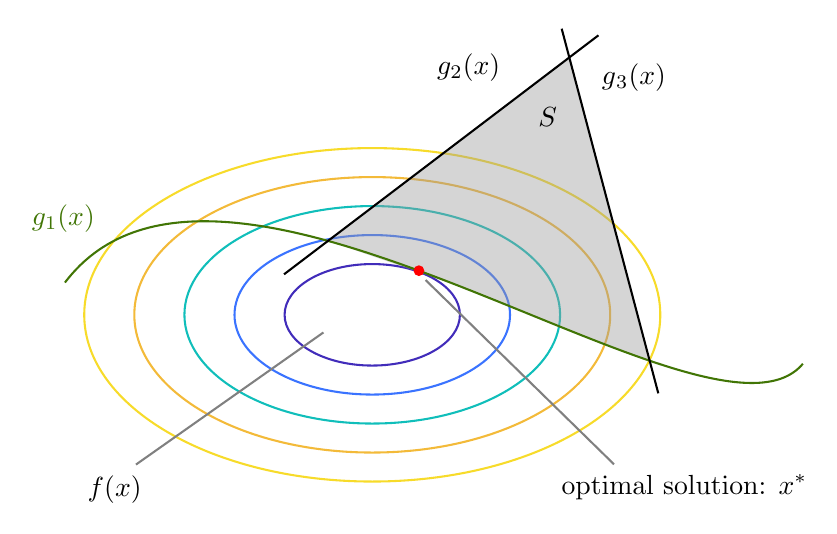
\begin{tikzpicture}[x=0.75pt,y=0.75pt,yscale=-1,xscale=1]

\draw  [color={rgb, 255:red, 16; green, 190; blue, 186 }  ,draw opacity=1 ] (109.02,186.67) .. controls (109.02,157.74) and (149.54,134.28) .. (199.52,134.28) .. controls (249.5,134.28) and (290.02,157.74) .. (290.02,186.67) .. controls (290.02,215.6) and (249.5,239.06) .. (199.52,239.06) .. controls (149.54,239.06) and (109.02,215.6) .. (109.02,186.67) -- cycle ;
\draw  [color={rgb, 255:red, 58; green, 115; blue, 255 }  ,draw opacity=1 ] (133.15,186.67) .. controls (133.15,165.45) and (162.87,148.25) .. (199.52,148.25) .. controls (236.17,148.25) and (265.89,165.45) .. (265.89,186.67) .. controls (265.89,207.89) and (236.17,225.09) .. (199.52,225.09) .. controls (162.87,225.09) and (133.15,207.89) .. (133.15,186.67) -- cycle ;
\draw  [color={rgb, 255:red, 65; green, 44; blue, 186 }  ,draw opacity=1 ] (157.28,186.67) .. controls (157.28,173.17) and (176.19,162.22) .. (199.52,162.22) .. controls (222.84,162.22) and (241.75,173.17) .. (241.75,186.67) .. controls (241.75,200.17) and (222.84,211.12) .. (199.52,211.12) .. controls (176.19,211.12) and (157.28,200.17) .. (157.28,186.67) -- cycle ;
\draw  [color={rgb, 255:red, 243; green, 186; blue, 57 }  ,draw opacity=1 ] (84.88,186.67) .. controls (84.88,150.02) and (136.21,120.31) .. (199.52,120.31) .. controls (262.83,120.31) and (314.16,150.02) .. (314.16,186.67) .. controls (314.16,223.32) and (262.83,253.03) .. (199.52,253.03) .. controls (136.21,253.03) and (84.88,223.32) .. (84.88,186.67) -- cycle ;
\draw  [color={rgb, 255:red, 247; green, 219; blue, 42 }  ,draw opacity=1 ] (60.75,186.67) .. controls (60.75,142.31) and (122.88,106.34) .. (199.52,106.34) .. controls (276.16,106.34) and (338.29,142.31) .. (338.29,186.67) .. controls (338.29,231.04) and (276.16,267) .. (199.52,267) .. controls (122.88,267) and (60.75,231.04) .. (60.75,186.67) -- cycle ;
\draw  [draw opacity=0][fill={rgb, 255:red, 155; green, 155; blue, 155 }  ,fill opacity=0.42 ] (294.71,62.79) .. controls (294.95,63.6) and (298.22,76.18) .. (302.64,93.2) .. controls (307.06,110.22) and (331.66,205.84) .. (332.57,207.79) .. controls (333.48,209.74) and (273,186.07) .. (256.43,178.79) .. controls (239.86,171.5) and (177.55,151.48) .. (178.57,150.64) .. controls (179.6,149.8) and (210.18,126.59) .. (238.44,105.22) .. controls (266.69,83.85) and (294.48,61.97) .. (294.71,62.79) -- cycle ;
\draw [color={rgb, 255:red, 65; green, 117; blue, 5 }  ,draw opacity=1 ]   (51.46,171.13) .. controls (127.5,70.75) and (363,262.75) .. (407,210.25) ;
\draw    (290.79,48.83) -- (337.33,224.5) ;
\draw    (157,167.17) -- (308.49,52.02) ;
\draw  [draw opacity=0][fill={rgb, 255:red, 255; green, 0; blue, 0 }  ,fill opacity=1 ] (219.42,165.4) .. controls (219.42,163.97) and (220.57,162.81) .. (222,162.81) .. controls (223.43,162.81) and (224.59,163.97) .. (224.59,165.4) .. controls (224.59,166.83) and (223.43,167.99) .. (222,167.99) .. controls (220.57,167.99) and (219.42,166.83) .. (219.42,165.4) -- cycle ;
\draw [color={rgb, 255:red, 128; green, 128; blue, 128 }  ,draw opacity=1 ]   (225.2,169.9) -- (316,258.7) ;
\draw [color={rgb, 255:red, 128; green, 128; blue, 128 }  ,draw opacity=1 ]   (85.67,258.83) -- (176,195.17) ;

\draw (278.02,85.14) node [anchor=north west][inner sep=0.75pt]    {$S$};
\draw (289.27,261.87) node [anchor=north west][inner sep=0.75pt]   [align=left] {optimal solution: $\displaystyle x^{*}$};
\draw (34,132.07) node [anchor=north west][inner sep=0.75pt]    {$\textcolor[rgb]{0.25,0.46,0.02}{g_{1}( x)}$};
\draw (229.33,59.4) node [anchor=north west][inner sep=0.75pt]    {$\textcolor[rgb]{0,0,0}{g_{2}( x)}$};
\draw (308.67,64.07) node [anchor=north west][inner sep=0.75pt]    {$\textcolor[rgb]{0,0,0}{g}\textcolor[rgb]{0,0,0}{_{3}}\textcolor[rgb]{0,0,0}{(}\textcolor[rgb]{0,0,0}{x}\textcolor[rgb]{0,0,0}{)}$};
\draw (60.93,262.67) node [anchor=north west][inner sep=0.75pt]   [align=left] {$\displaystyle f( x)$};


\end{tikzpicture}
\section{Quadratic Programming\label{sec:qp}}
The optimization problem \eqref{eq:optmization_problem_def_real} is called a \emph{quadratic program} (QP) if the objective is convex quadratic and the constrain functions are affine. We express a quadratic program problem in the following form:
\begin{IEEEeqnarray}{cc}
\phantomsection \label{eq:qp} \IEEEyesnumber \IEEEyessubnumber*
\; \; \minimize_x \; \; & \frac{1}{2} x^\top P x + q^\top x + r\\
\st & G x \preceq h.
\end{IEEEeqnarray}
$x\in\mathbb{R}^n$, $P \succ 0$ is a positive definite matrix, $q\in \mathbb{R}^n$, $G\in \mathbb{R}^{m \times n}$, $h\in \mathbb{R}^m$ and $r\in\mathbb{R}$.
\begin{figure}[t]
\centering
    \begin{subfigure}[b]{0.48\textwidth}
        \centering
        \includegraphics{chapter_optimization_introduction/figures/qp_active.tikz}
        \caption{Optimizer on boundary of $S$.}
        \label{fig:qp_active}
    \end{subfigure}
    \hfill
    \begin{subfigure}[b]{0.48\textwidth}
        \centering
        \includegraphics{chapter_optimization_introduction/figures/qp.tikz}
        \caption{Optimizer in interior of $S$.}
        \label{fig:qp}
    \end{subfigure}
	\caption[Solution of a QP problem]{Geometric interpretation of the QP solution. (a) The solution belongs to the boundary of $P$. One of the constraint is active (green line). (b) The solution belongs to the interior of $P$. In this case, $x^* = -P^{-1} q$.}
	\label{fig:qp_active_qp}
\end{figure}
If the set $S = \{x | G x \preceq h\}$ is not empty, the solution exists and is unique. 
Figure~\eqref{fig:qp_active_qp} illustrates the solution of a QP problem. In Figure~\eqref{fig:qp_active} the optimal solution belongs to the boundary of the feasible set $S$, while in Figure~\eqref{fig:qp} the solution belongs to the interior of $S$. In this case, the optimization problem~\eqref{eq:qp} is equivalent to an unconstrained optimization problem. Since the cost function is quadratic and hence convex, the optimal solution is given by setting the gradient of 
$\frac{1}{2} x^\top P x + q^\top x + r$ to zero:
\begin{equation}
    \nabla_x \left[\frac{1}{2} x^\top P x + q^\top x + r \right] = 0,
\end{equation}
whose solution is given by $x^* = -P^{-1} q$.

\paragraph{Dual of QP}
Consider~\eqref{eq:qp} the Lagrange function~\eqref{eq:lagrangian_function} is given by
\begin{equation}
    \label{eq:lagrangian_function_qp}
    \mathcal{L}(x, \lambda) = x^\top P x + q^\top x  - \lambda ^\top \left[ Gx -h \right],
\end{equation}
The dual cost~\eqref{eq:dual_function} is obtained by minimizing the Lagrange function~\eqref{eq:lagrangian_function_qp} with respect to $x$
\begin{equation}
\label{eq:dual_cost_qp}
    g(\lambda) = \min_x \left\{ x^\top P x + q^\top x  - \lambda ^\top \left[ Gx -h \right] \right\},
\end{equation}
For a given $\lambda$, the Lagrange function~\eqref{eq:lagrangian_function_qp} is convex, consequently the dual cost~\eqref{eq:dual_cost_qp} is obtained by setting the gradient of~\eqref{eq:lagrangian_function_qp} equal to zero. We then have
\begin{equation}
    \label{eq:x_qp_dual}
    x = -P^{-1} \left(q + G^\top \lambda\right).
\end{equation}
Finally, the dual problem~\eqref{eq:lagrangian_dual_problem} is given by substituting~\eqref{eq:x_qp_dual} into~\eqref{eq:dual_cost_qp} and computing the maximum for $\lambda \succeq 0_{m\times1}$ as
\begin{IEEEeqnarray}{cl}
\label{eq:lagrangian_dual_problem_qp} \IEEEyesnumber \IEEEyessubnumber*
\; \; \minimize\limits_{\lambda} \; \; & \frac{1}{2} \lambda^\top (G P^{-1} G^\top) \lambda + \lambda^\top(h - G P^{-1} q) + \frac{1}{2} q^\top H^{-1} q \\
\st & \lambda \succeq 0_{m\times1}.
\end{IEEEeqnarray}
The dual of a QP problem is a QP problem itself.

\paragraph{KKT of QP}
Given a QP problem~\eqref{eq:lagrangian_function_qp} the KKT conditions~\eqref{eq:kkt} become
\begin{IEEEeqnarray}{rl}
\phantomsection \label{eq:kkt_qp} \IEEEyesnumber \IEEEyessubnumber*
Px + q + G^\top \lambda &= 0 \\
\lambda^{* ^\top} (G x - h) &= 0 \\
\lambda^{*} &\succeq 0_{ m \times1}  \\
G x - h  &\preceq 0_{ m \times1}.
\end{IEEEeqnarray}

\section{Optimal control\label{sec:optimal_control}}
Let us consider a dynamical system 
\begin{equation}
    \label{eq:oc_dynamical_system}
    \dot{x}(t) = f(x(t), u(t), t),
\end{equation}
where $x(t) \in \mathbb{R}^n$ is the state of the dynamical system and $u(t) \in \mathcal{U} \subseteq \mathbb{R}^m$ is the control input. 
Our aim is to determine the evolution of the system given an initial value $x(0) = x_0$. Such a problem is often known as \emph{Initial Value Problem}, denoted as IVP. If the terminal condition is also specified, $x(t_f) = x_f$, we name the problem \emph{Boundary Value Problem} (BVT).
\par
If the control input $u(t)$ is known and is sufficiently regular, the IVP has an unique solution that depends on the control history $u(t)$.
\par
In more complex scenarios, the dynamical system~\eqref{eq:oc_dynamical_system} is extended with a set of algebraic constraints of the form
\begin{equation}
    \label{eq:oc_constraint}
    c(x(t), u(t), t) \le 0_{n_c \times 1}.
\end{equation}
The dynamical system~\eqref{eq:oc_dynamical_system} together with~\eqref{eq:oc_constraint} define a \emph{Differential Algebraic Equation} (DAE).
\par
Let us now introduce a cost function whose purpose is to evaluate the performance index of a control input sequence $u$ in a closed interval $t\in[t_0, t_f]$. We define a \emph{performance functional index}, or simply \emph{cost function}, denoted as $\mathcal{J}(x_0, u(.), t)$ as:
\begin{equation}
    \label{eq:oc_cost_function}
    \mathcal{J}\left(x_0, u(.), t \right) = \beta(x(t_f), t_f) + \int_{t_0} ^{t_f} \ell\left(x(\tau), u(\tau), \tau\right) \diff \tau,
\end{equation}
where $\beta(x(t_f), t_f)$ is called \emph{Mayer} term and weighs the terminal state. While $\ell\left(x(\tau), u(\tau), \tau\right)$ is the \emph{Lagrange} term. The Mayer term is also known as \emph{terminal cost}, and weighs the state of the system at $t = t_f$. On the other hand, the Lagrange term, also known as \emph{running cost}, weighs the path to reach the final state.
\par
Combining the dynamical system \eqref{eq:oc_dynamical_system}, the algebraic constraint \eqref{eq:oc_constraint}, and the cost function \eqref{eq:oc_cost_function} we define the optimal control problem (OCP) as follows
\begin{IEEEeqnarray}{cll}
\phantomsection \label{eq:oc_bolza} \IEEEyesnumber \IEEEyessubnumber*
\; \; \minimize\limits_{u\in\mathcal{U}} \; \;   &  \IEEEeqnarraymulticol{2}{l}{\beta(x(t_f), t_f) + \int_{t_0} ^{t_f} \ell\left(x(\tau), u(\tau), \tau\right) \diff \tau} \label{eq:oc_bolza_cost} \\ 
\st &  \dot{x}(t) = f(x(t), u(t), t)  & \quad \quad t \in [t_0, t_f] \\
&  c(x(t), u(t), t) \le 0_{n_c \times 1} & \quad \quad t \in [t_0, t_f] \label{eq:oc_bolza_constraint} \\
& x(t_0) = x_0. &
\end{IEEEeqnarray}
The optimal control problem~\eqref{eq:oc_bolza} is known as \emph{Bolza} optimization problem.  We recall that an OCP can be written in three forms, namely: \emph{Bolza}, \emph{Mayer} and \emph{Lagrange} forms.   
They apparently differ in the formulation of the functional to be optimized, but it is worth noticing that they are equivalent and that it is possible to convert each problem into the other two forms.
If the integral term in the cost function~\eqref{eq:oc_bolza_cost} is set to zero, the problem is said to be written in \emph{Mayer} form. On the other hand, if the terminal cost in~\eqref{eq:oc_bolza_cost} is set to zero, the problem is in Lagrange form. \par
The OCP~\eqref{eq:oc_bolza} is normally solved by applying three different strategies. The \emph{dynamic programming}~\citep{Bellman1952OnProgramming,Tawiah2021OptimalProgramming}, the \emph{indirect methods}~\citep{Liberzon2012CalculusTheory,Bertolazzi2005SymbolicNumericSystems,Pontriagin1962TheProcesses} or the \emph{direct methods}~\citep{BettsPractical2010}.


\paragraph{Dynamic programming}
The dynamic programming (DP) methodology attempts to analytically find the optimal control strategy by breaking the OCP into smaller subproblems applying the \emph{Bellman's principle of optimality}~\citep{Gross2016OnOptimality,Bellman1952OnProgramming,Dreyfus2002RichardProgramming}:
\begin{center}
\begin{minipage}{12cm}
   \emph{An optimal policy has the property that whatever the initial state and initial decision are, the remaining decisions must constitute an optimal policy with regard to the state resulting from the first decision.}
\end{minipage}
\end{center}
Since we do not exploit the \emph{dynamic programming} techniques for the rest of the thesis, we avoid further discussing these methods.
\paragraph{Indirect methods}
The indirect methods are another class of analytical optimization methods. Unlike DP, they rely on the \emph{Pontryagin’s minimum principle}~\citep[Section~5.3]{kirk2012optimal} to compute the optimality conditions. The methods exploit the Hamiltonian function introduced for the Hamilton-Jacobi-Bellman equation to reduce the solution of the OCP to the solution of a $2n$ equations given in the form of a two-point boundary value problem. Since we do not exploit \emph{Indirect methods}for the rest of the thesis, we will not further discuss them.
\paragraph{Direct methods}
Finally, in the direct method approach, the OCP is discretized, \emph{transcribed} into a nonlinear programming problem, and finally solved numerically. 
\par
In this thesis, we approach the OCP only by applying direct methods. Section~\ref{sec:direct_methods} presents the common integration methods exploited to convert the continuous dynamics~\eqref{eq:oc_dynamical_system} into a discrete one of the form
\begin{equation}
    x(t+\delta t) = \Gamma(x(t), u(t), t).
\end{equation}

\subsection{Direct methods\label{sec:direct_methods}}
Given an optimization problem~\eqref{eq:oc_bolza}, our objective is to transcribe it into a nonlinear programming problem of the form~\eqref{eq:optmization_problem_def}. Even if the formulation in~\eqref{eq:oc_bolza} seems to be similar to~\eqref{eq:optmization_problem_def}, it is worth recalling some main differences. In an OCP, we seek a control strategy $u(t)$ where $t$ belongs to a close interval. $u(t)$ is in general a function that may depend on the state of the system. On the other hand, the outcome of a nonlinear optimization problem~\eqref{eq:optmization_problem_def} is just a sequence of control actions. Furthermore, the nonlinear optimization problem~\eqref{eq:optmization_problem_def} is completely agnostic to the concept of time evolution of the dynamical system~\eqref{eq:oc_dynamical_system}. These two main differences are overcome by discretizing the dynamics of the continuous system.

\subsubsection{Discretization of the dynamical system}
We call the solution of the dynamics equation~\eqref{eq:oc_dynamical_system}, the \emph{state transition function} 
\begin{equation}
    \label{eq:oc_dynamical_system_solution}
    x(t) = \phi(x_0, t_0, u).
\end{equation}
We want to transform it into discrete difference equations, suitable for numerical computing.  We now introduce the notation $x_k$ as the value of a variable $x$ evaluated at $t_0 + k \diff t$, i.e., $x_k = x(t_0 + k \diff t)$. We approximate the state evolution of~\eqref{eq:oc_dynamical_system} with
\begin{equation}
\label{eq:oc_discretization_solution}
x_{k+1} = \Gamma \left(x_k, u_k, k\right).
\end{equation}
where $\Gamma: \mathbb{R}^{n} \times \mathbb{R}^m \times \mathbb{N}  \rightarrow \mathbb{R}^{n}$. It is worth noting that, by recursively applying~\eqref{eq:oc_discretization_solution} from $k = 0$ to $k = N$, \eqref{eq:oc_discretization_solution} is the discrete approximation of~\eqref{eq:oc_dynamical_system_solution}.  $N = (t_f - t_0) / \diff t$ is often denoted as \emph{time horizon}.
\paragraph{Forward Euler}
The most common \emph{single-step} method is the \emph{forward Euler} integration scheme:
\begin{equation}
    \label{eq:forward_euler}
	x_{k+1} = x_k  + \diff t f\left(x_k, u_k, t_k\right).
\end{equation}
It is worth noting that, for sufficiently high $\diff t$, the forward Euler method is subject to numerical instability.

\paragraph{Backward Euler} 
Given a dynamical system~\eqref{eq:oc_dynamical_system} the \emph{backward Euler} method gives the following approximation 
\begin{equation} 
    \label{eq:backward_euler}
	x_{k+1} = x_k  + \diff t f\left(x_{k+1}, u_{k+1}, t_{k+1}\right).
\end{equation}
The backward Euler is an \emph{implicit single step} method. As a consequence, it is numerically stable independently from the chosen time step \citep{Ascher1997Implicit-explicitEquations}. 
Given the presence of $x_{k+1}$ in both sizes of~\eqref{eq:backward_euler} it would be necessary to numerically solve~\eqref{eq:backward_euler} to find an explicit expression of $x_{k+1}$ as a function of $x_{k}$, $u_{k}$, and $t_{k}$.

\paragraph{Tustin integration method}
The \emph{Tustin integration} also known \emph{trapezoidal} method is another implicit method of the form:
\begin{equation}
    \label{eq:trapezoidal}
	x_{k+1} = x_k + \frac{\diff t}{2} \left[f\left(k_k, u_k, t_k\right) + f\left(x_{k+1}, u_{k+1}, t_{k+1}\right) \right].
\end{equation}
Unlike Euler's methods, the trapezoidal method considers the dynamics at two time instants, $k$ and $k+1$. For this reason, the trapezoidal method is considered a \emph{multiple collocations} method.
We finally recall that the trapezoidal method~\eqref{eq:trapezoidal} gives a better approximation of the Euler methods~\eqref{eq:forward_euler}~\eqref{eq:backward_euler}.

\paragraph{Zero order hold\label{sec:zoh}}
Let us now assume that the dynamical system~\eqref{eq:oc_dynamical_system} is described by linear time-invariant ordinary differential equations of the form
\begin{equation}
    \label{eq:lti}
    \dot{x}(t) = A x(t) + B u(t).
\end{equation}
Where $A \in \mathbb{R}^{n \times n}$ and $B \in \mathbb{R}^{n \times m}$ and $x(t_0) = x_0$. The system \eqref{eq:lti} admits a closed form solution~\eqref{eq:oc_dynamical_system_solution} of the form
\begin{equation}
    \label{eq:lti_solution}
x(t) = e^{A (t-t_0)} x_0 + \int_{t_0}^{t} e ^{A(t - \tau)} B u(\tau) \diff \tau
\end{equation}
Let us now assume that the control input is kept constant in an interval $\diff t$, i.e., $u(t) = \bar{u}$ for $t \in [t_0,  t_0 + \diff t]$. Then Equation~\eqref{eq:lti_solution} can be rewritten as
\begin{equation}
\label{eq:lti_solution_1}
x(t_0 + \diff t) = e^{A (\diff t)} x_0 + \int_{0}^{\diff t} e ^{A \tau} \diff \tau B \bar{u}
\end{equation}
Assume that the control input is kept constant during every sampling period $\diff t$, and that its value is equal to $u(t_0 + k \diff t) = u_k$. Then Equation \eqref{eq:lti_solution_1} can be rewritten as 
\begin{IEEEeqnarray}{ll}
\phantomsection \label{eq:lti_solution_discrete} \IEEEyesnumber \IEEEyessubnumber*
x_{k+1} &= e^{A \diff t} x_k + \int_{0}^{\diff t} e ^{A \tau} \diff \tau B u_k \\
& = A_d x_k + B_d u_k.
\end{IEEEeqnarray}
This method is known as the \emph{zero order hold} integration method since the input is kept constant (i.e., it is held) during the sampling period. 
\par
The presented integration methods can be exploited recursively to determine the state evolution from $t_0$ to $t_f$. Consequently, it would be possible to convert the continuous dynamical system into a set of equality constraints that can be embedded in the optimization problem~\eqref{eq:optmization_problem_def}. This technique is often denoted as \emph{shooting}.

\subsection{Shooting methods\label{sec:shooting_methods}}
\begin{figure}[t]
\centering
    \begin{subfigure}[b]{1\textwidth}
        \centering
        \includegraphics{chapter_optimization_introduction/figures/single_shooting.tikz}
        \caption{Single shooting.}
        \label{fig:single_shooting}
    \end{subfigure}
    \hfill
    \begin{subfigure}[b]{1\textwidth}
        \centering
        \includegraphics{chapter_optimization_introduction/figures/multiple_shooting.tikz}
        \caption{Multiple shooting.}
        \label{fig:multiple_shooting}
    \end{subfigure}
	\caption[Single and Multiple shooting]{Single and Multiple shooting.}
	\label{fig:shooting}
\end{figure}
\subsubsection{Single shooting}
Let us consider the discretized dynamical system~\eqref{eq:oc_discretization_solution}. We notice that a given state $x_{k+1}$ can be written as a function of the initial state $x_0$ and the input sequence $u_j$ where $j \in [0, k]$. In fact,
\begin{IEEEeqnarray*}{rcl}
\phantomsection \label{eq:ss_dynamics} \IEEEyesnumber \IEEEyessubnumber*
    x_1 &=& \Gamma(x_0, u_0), \\
    x_2 &=& \Gamma(x_1, u_1) = \Gamma\left(\Gamma(x_0, u_0), u_1\right), \\
    x_4 &=& \Gamma(x_2, u_2) = \Gamma\left(\Gamma\left(\Gamma(x_0, u_0), u_1\right), u_2\right), \\
    \IEEEeqnarraymulticol{3}{c}{\vdots}\\
	x_{k+1} &=& \Gamma(x_k, u_k) = \Gamma\left(\hdots\left(\Gamma(x_0, u_0), \hdots \right), u_k\right).
\end{IEEEeqnarray*}
Therefore, with a \emph{single shooting} method, it is possible to obtain the terminal state starting from the initial one, without having to consider all the intermediate states. In an optimization framework, the set of optimization variables would consist only of the control inputs applied at each step. 


\subsubsection{Multiple shooting}
If the system is nonlinear, the composition of function $\Gamma$ $N$ times may result in a very complex expression. In addition, it is difficult to specify \emph{path} constraints, i.e., those involving intermediate states. These problems, typical of the method just introduced, are solved using a \emph{multiple shooting} approach~\citep{Bock84,diehl2006fast}, where all the intermediate state variables are also optimization variables. This has the clear disadvantage of including more variables and constraints in the optimization problem. In fact, it is necessary to add a constraint for each pair of optimization variables of the form
\begin{IEEEeqnarray}{c}
\phantomsection \label{eq:ms_dynamics} \IEEEyesnumber \IEEEyessubnumber*
    x_1 - \Gamma(x_0, u_0) = 0 \\
    x_2 - \Gamma(x_1, u_2) = 0 \\
    x_3 - \Gamma(x_2, u_2) = 0 \\
    \vdots\\
	x_{N} - \Gamma(x_{N-1}, u_{N-1}) = 0.
\end{IEEEeqnarray}
Where each constraint $i$ depends only on the state $i$ , $i+1$ and the control input $i$. Seeing that the dynamics is discretized, the cost function~\eqref{eq:oc_bolza_cost} becomes 
\begin{equation}
\label{eq:ms_cost}
	\mathcal{J}\left(x_0, \hdots, x_{N}, u_0, \hdots, u_{N-1} \right) = \beta\left(x_{N}\right) + \sum_i^{N - 1} \ell \left(x_i, u_i\right) \diff t.
\end{equation}
Following the same approach, the algebraic constraints~\eqref{eq:oc_bolza_constraint}, become a list of constraints
\begin{IEEEeqnarray}{c}
\phantomsection \label{eq:ms_constraints} \IEEEyesnumber \IEEEyessubnumber*
c(x_0, u_0) \le 0_{n_c \times 1} \\
c(x_1, u_1) \le 0_{n_c \times 1} \\
c(x_2, u_2) \le 0_{n_c \times 1} \\
    \vdots\\
c(x_{N-1}, u_{N-1}) \le 0_{n_c \times 1}.
\end{IEEEeqnarray}

Substituting the discretized dynamics~\eqref{eq:ms_dynamics}, the cost function~\eqref{eq:ms_cost} and algebraic constraints~\eqref{eq:ms_constraints} into the Bolza problem~\eqref{eq:oc_bolza}, we obtain the final form of the optimal control problem solved with a direct multiple shooting method  
\begin{IEEEeqnarray}{cll}
\phantomsection \label{eq:mc_oc} \IEEEyesnumber \IEEEyessubnumber*
\; \; \minimize\limits_{x_0, \hdots, x_{N}, u_0, \hdots, u_{N-1}} \; \;   &  \IEEEeqnarraymulticol{2}{l}{\beta\left(x_{N}\right) + \sum_k^{N - 1} \ell \left(x_k, u_k\right) \diff t} \\ 
\st &  x_{k+1} - \Gamma(x_k, u_k) = 0 & \quad \quad k = 0\hdots N-1 \\
& c(x_k, u_k) \le 0_{n_c \times 1} & \quad \quad k = 0\hdots N-1 \\
&  x_0 = x(t_0).
\end{IEEEeqnarray}


\tikzset{every picture/.style={line width=0.75pt}} %

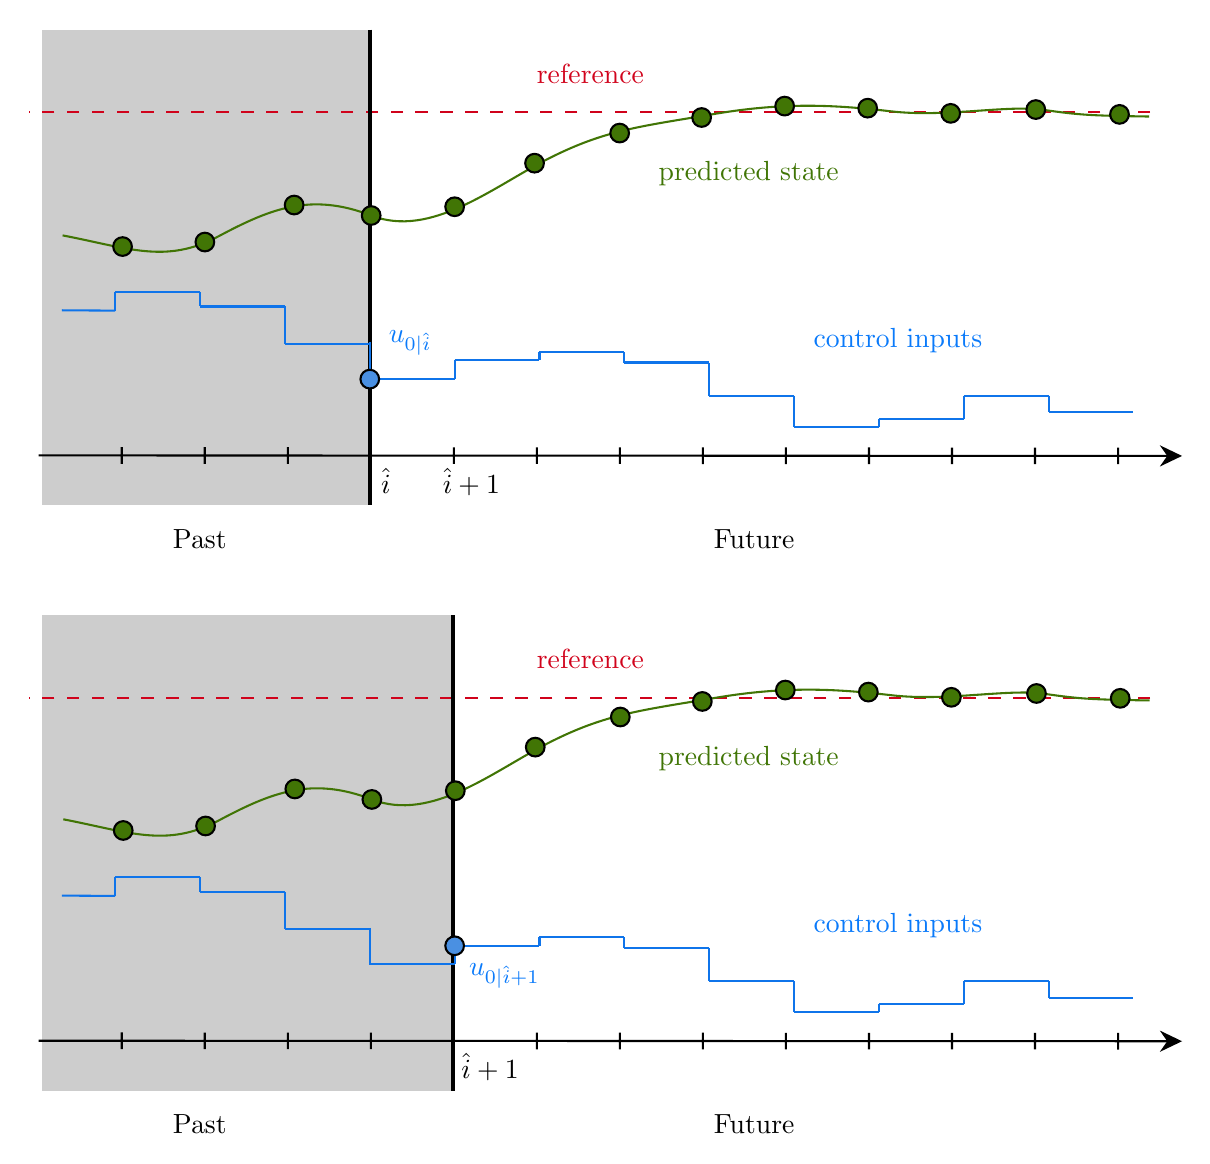
\begin{tikzpicture}[x=0.75pt,y=0.75pt,yscale=-1,xscale=1]

\draw  [draw opacity=0][fill={rgb, 255:red, 155; green, 155; blue, 155 }  ,fill opacity=0.5 ] (17,34.67) -- (176,34.67) -- (176,263.75) -- (17,263.75) -- cycle ;
\draw [color={rgb, 255:red, 208; green, 2; blue, 27 }  ,draw opacity=1 ][line width=0.75]  [dash pattern={on 4.5pt off 4.5pt}]  (551,74.45) -- (10.67,74.45) ;
\draw [line width=1.5]    (175,34.67) -- (175,263.75) ;
\draw [color={rgb, 255:red, 65; green, 117; blue, 5 }  ,draw opacity=1 ]   (27,133.75) .. controls (58.62,139.8) and (76.71,147.73) .. (102,134.25) .. controls (127.29,120.77) and (146.69,112.96) .. (175.67,124.17) .. controls (204.65,135.38) and (234.43,110.24) .. (261.71,96.45) .. controls (289,82.67) and (306.33,81.17) .. (341,75.25) .. controls (375.67,69.33) and (400.33,71) .. (426.33,74) .. controls (452.33,77) and (482.21,70.78) .. (499.5,73.25) .. controls (516.79,75.72) and (521.1,76.02) .. (550.43,76.48) ;
\draw  [fill={rgb, 255:red, 65; green, 117; blue, 5 }  ,fill opacity=1 ] (91.05,136.95) .. controls (91.05,134.47) and (93.06,132.45) .. (95.55,132.45) .. controls (98.03,132.45) and (100.05,134.47) .. (100.05,136.95) .. controls (100.05,139.44) and (98.03,141.45) .. (95.55,141.45) .. controls (93.06,141.45) and (91.05,139.44) .. (91.05,136.95) -- cycle ;
\draw  [fill={rgb, 255:red, 65; green, 117; blue, 5 }  ,fill opacity=1 ] (51.38,139.12) .. controls (51.38,136.64) and (53.4,134.62) .. (55.88,134.62) .. controls (58.37,134.62) and (60.38,136.64) .. (60.38,139.12) .. controls (60.38,141.61) and (58.37,143.62) .. (55.88,143.62) .. controls (53.4,143.62) and (51.38,141.61) .. (51.38,139.12) -- cycle ;
\draw  [fill={rgb, 255:red, 65; green, 117; blue, 5 }  ,fill opacity=1 ] (134.05,119.12) .. controls (134.05,116.64) and (136.06,114.62) .. (138.55,114.62) .. controls (141.03,114.62) and (143.05,116.64) .. (143.05,119.12) .. controls (143.05,121.61) and (141.03,123.62) .. (138.55,123.62) .. controls (136.06,123.62) and (134.05,121.61) .. (134.05,119.12) -- cycle ;
\draw  [fill={rgb, 255:red, 65; green, 117; blue, 5 }  ,fill opacity=1 ] (171.17,124.17) .. controls (171.17,121.68) and (173.18,119.67) .. (175.67,119.67) .. controls (178.15,119.67) and (180.17,121.68) .. (180.17,124.17) .. controls (180.17,126.65) and (178.15,128.67) .. (175.67,128.67) .. controls (173.18,128.67) and (171.17,126.65) .. (171.17,124.17) -- cycle ;
\draw  [fill={rgb, 255:red, 65; green, 117; blue, 5 }  ,fill opacity=1 ] (211.38,119.95) .. controls (211.38,117.47) and (213.4,115.45) .. (215.88,115.45) .. controls (218.37,115.45) and (220.38,117.47) .. (220.38,119.95) .. controls (220.38,122.44) and (218.37,124.45) .. (215.88,124.45) .. controls (213.4,124.45) and (211.38,122.44) .. (211.38,119.95) -- cycle ;
\draw  [fill={rgb, 255:red, 65; green, 117; blue, 5 }  ,fill opacity=1 ] (249.88,98.95) .. controls (249.88,96.47) and (251.9,94.45) .. (254.38,94.45) .. controls (256.87,94.45) and (258.88,96.47) .. (258.88,98.95) .. controls (258.88,101.44) and (256.87,103.45) .. (254.38,103.45) .. controls (251.9,103.45) and (249.88,101.44) .. (249.88,98.95) -- cycle ;
\draw  [fill={rgb, 255:red, 65; green, 117; blue, 5 }  ,fill opacity=1 ] (290.88,84.45) .. controls (290.88,81.97) and (292.9,79.95) .. (295.38,79.95) .. controls (297.87,79.95) and (299.88,81.97) .. (299.88,84.45) .. controls (299.88,86.94) and (297.87,88.95) .. (295.38,88.95) .. controls (292.9,88.95) and (290.88,86.94) .. (290.88,84.45) -- cycle ;
\draw  [fill={rgb, 255:red, 65; green, 117; blue, 5 }  ,fill opacity=1 ] (330.38,76.95) .. controls (330.38,74.47) and (332.4,72.45) .. (334.88,72.45) .. controls (337.37,72.45) and (339.38,74.47) .. (339.38,76.95) .. controls (339.38,79.44) and (337.37,81.45) .. (334.88,81.45) .. controls (332.4,81.45) and (330.38,79.44) .. (330.38,76.95) -- cycle ;
\draw  [fill={rgb, 255:red, 65; green, 117; blue, 5 }  ,fill opacity=1 ] (370.38,71.45) .. controls (370.38,68.97) and (372.4,66.95) .. (374.88,66.95) .. controls (377.37,66.95) and (379.38,68.97) .. (379.38,71.45) .. controls (379.38,73.94) and (377.37,75.95) .. (374.88,75.95) .. controls (372.4,75.95) and (370.38,73.94) .. (370.38,71.45) -- cycle ;
\draw  [fill={rgb, 255:red, 65; green, 117; blue, 5 }  ,fill opacity=1 ] (410.38,72.45) .. controls (410.38,69.97) and (412.4,67.95) .. (414.88,67.95) .. controls (417.37,67.95) and (419.38,69.97) .. (419.38,72.45) .. controls (419.38,74.94) and (417.37,76.95) .. (414.88,76.95) .. controls (412.4,76.95) and (410.38,74.94) .. (410.38,72.45) -- cycle ;
\draw  [fill={rgb, 255:red, 65; green, 117; blue, 5 }  ,fill opacity=1 ] (450.38,74.95) .. controls (450.38,72.47) and (452.4,70.45) .. (454.88,70.45) .. controls (457.37,70.45) and (459.38,72.47) .. (459.38,74.95) .. controls (459.38,77.44) and (457.37,79.45) .. (454.88,79.45) .. controls (452.4,79.45) and (450.38,77.44) .. (450.38,74.95) -- cycle ;
\draw  [fill={rgb, 255:red, 65; green, 117; blue, 5 }  ,fill opacity=1 ] (491.38,73.12) .. controls (491.38,70.64) and (493.4,68.62) .. (495.88,68.62) .. controls (498.37,68.62) and (500.38,70.64) .. (500.38,73.12) .. controls (500.38,75.61) and (498.37,77.62) .. (495.88,77.62) .. controls (493.4,77.62) and (491.38,75.61) .. (491.38,73.12) -- cycle ;
\draw  [fill={rgb, 255:red, 65; green, 117; blue, 5 }  ,fill opacity=1 ] (531.71,75.45) .. controls (531.71,72.97) and (533.73,70.95) .. (536.21,70.95) .. controls (538.7,70.95) and (540.71,72.97) .. (540.71,75.45) .. controls (540.71,77.94) and (538.7,79.95) .. (536.21,79.95) .. controls (533.73,79.95) and (531.71,77.94) .. (531.71,75.45) -- cycle ;
\draw    (15.5,239.75) -- (563.33,240) (55.5,235.77) -- (55.5,243.77)(95.5,235.79) -- (95.5,243.79)(135.5,235.8) -- (135.5,243.8)(175.5,235.82) -- (175.5,243.82)(215.5,235.84) -- (215.5,243.84)(255.5,235.86) -- (255.5,243.86)(295.5,235.88) -- (295.5,243.88)(335.5,235.9) -- (335.5,243.9)(375.5,235.91) -- (375.5,243.91)(415.5,235.93) -- (415.5,243.93)(455.5,235.95) -- (455.5,243.95)(495.5,235.97) -- (495.5,243.97)(535.5,235.99) -- (535.5,243.99) ;
\draw [shift={(566.33,240)}, rotate = 180.03] [fill={rgb, 255:red, 0; green, 0; blue, 0 }  ][line width=0.08]  [draw opacity=0] (10.72,-5.15) -- (0,0) -- (10.72,5.15) -- (7.12,0) -- cycle    ;
\draw [color={rgb, 255:red, 15; green, 116; blue, 234 }  ,draw opacity=1 ]   (175,203) -- (215.88,203) ;
\draw [color={rgb, 255:red, 15; green, 116; blue, 234 }  ,draw opacity=1 ]   (215.88,194) -- (256.76,194) ;
\draw [color={rgb, 255:red, 15; green, 116; blue, 234 }  ,draw opacity=1 ]   (256.76,190) -- (297.64,190) ;
\draw [color={rgb, 255:red, 15; green, 116; blue, 234 }  ,draw opacity=1 ]   (297.64,195) -- (338.52,195) ;
\draw [color={rgb, 255:red, 15; green, 116; blue, 234 }  ,draw opacity=1 ]   (338.52,211) -- (379.4,211) ;
\draw [color={rgb, 255:red, 15; green, 116; blue, 234 }  ,draw opacity=1 ]   (379.4,226) -- (420.29,226) ;
\draw [color={rgb, 255:red, 15; green, 116; blue, 234 }  ,draw opacity=1 ]   (420.29,222) -- (461.17,222) ;
\draw [color={rgb, 255:red, 15; green, 116; blue, 234 }  ,draw opacity=1 ]   (461.17,211) -- (502.05,211) ;
\draw [color={rgb, 255:red, 15; green, 116; blue, 234 }  ,draw opacity=1 ]   (502.05,219) -- (542.93,219) ;
\draw [color={rgb, 255:red, 15; green, 116; blue, 234 }  ,draw opacity=1 ]   (134.12,186) -- (175,186) ;
\draw [color={rgb, 255:red, 15; green, 116; blue, 234 }  ,draw opacity=1 ]   (93.24,168) -- (134.12,168) ;
\draw [color={rgb, 255:red, 15; green, 116; blue, 234 }  ,draw opacity=1 ]   (52.36,161) -- (93.24,161) ;
\draw [color={rgb, 255:red, 15; green, 116; blue, 234 }  ,draw opacity=1 ]   (26.67,169.83) -- (52.36,170) ;
\draw [color={rgb, 255:red, 15; green, 116; blue, 234 }  ,draw opacity=1 ]   (93.24,161) -- (93.24,168) ;
\draw [color={rgb, 255:red, 15; green, 116; blue, 234 }  ,draw opacity=1 ]   (52.36,161) -- (52.36,170) ;
\draw [color={rgb, 255:red, 15; green, 116; blue, 234 }  ,draw opacity=1 ]   (134.12,168) -- (134.12,186) ;
\draw [color={rgb, 255:red, 15; green, 116; blue, 234 }  ,draw opacity=1 ]   (175,185.33) -- (175,203.33) ;
\draw [color={rgb, 255:red, 15; green, 116; blue, 234 }  ,draw opacity=1 ]   (215.88,194) -- (215.88,203) ;
\draw [color={rgb, 255:red, 15; green, 116; blue, 234 }  ,draw opacity=1 ]   (461.17,211) -- (461.17,222) ;
\draw [color={rgb, 255:red, 15; green, 116; blue, 234 }  ,draw opacity=1 ]   (256.76,190) -- (256.76,194) ;
\draw [color={rgb, 255:red, 15; green, 116; blue, 234 }  ,draw opacity=1 ]   (297.64,190) -- (297.64,195) ;
\draw [color={rgb, 255:red, 15; green, 116; blue, 234 }  ,draw opacity=1 ]   (338.52,195) -- (338.52,211) ;
\draw [color={rgb, 255:red, 15; green, 116; blue, 234 }  ,draw opacity=1 ]   (379.4,211) -- (379.4,226) ;
\draw [color={rgb, 255:red, 15; green, 116; blue, 234 }  ,draw opacity=1 ]   (420.29,222) -- (420.29,226) ;
\draw [color={rgb, 255:red, 15; green, 116; blue, 234 }  ,draw opacity=1 ]   (502.05,211) -- (502.05,219) ;
\draw  [draw opacity=0][fill={rgb, 255:red, 155; green, 155; blue, 155 }  ,fill opacity=0.5 ] (17,316.67) -- (215,316.67) -- (215,545.75) -- (17,545.75) -- cycle ;
\draw [color={rgb, 255:red, 208; green, 2; blue, 27 }  ,draw opacity=1 ][line width=0.75]  [dash pattern={on 4.5pt off 4.5pt}]  (551,356.45) -- (10.67,356.45) ;
\draw [line width=1.5]    (215,316.67) -- (215,545.75) ;
\draw    (15.5,521.75) -- (563.33,522) (55.5,517.77) -- (55.5,525.77)(95.5,517.79) -- (95.5,525.79)(135.5,517.8) -- (135.5,525.8)(175.5,517.82) -- (175.5,525.82)(215.5,517.84) -- (215.5,525.84)(255.5,517.86) -- (255.5,525.86)(295.5,517.88) -- (295.5,525.88)(335.5,517.9) -- (335.5,525.9)(375.5,517.91) -- (375.5,525.91)(415.5,517.93) -- (415.5,525.93)(455.5,517.95) -- (455.5,525.95)(495.5,517.97) -- (495.5,525.97)(535.5,517.99) -- (535.5,525.99) ;
\draw [shift={(566.33,522)}, rotate = 180.03] [fill={rgb, 255:red, 0; green, 0; blue, 0 }  ][line width=0.08]  [draw opacity=0] (10.72,-5.15) -- (0,0) -- (10.72,5.15) -- (7.12,0) -- cycle    ;
\draw [color={rgb, 255:red, 15; green, 116; blue, 234 }  ,draw opacity=1 ]   (175,485) -- (215.88,485) ;
\draw [color={rgb, 255:red, 15; green, 116; blue, 234 }  ,draw opacity=1 ]   (215.88,476) -- (256.76,476) ;
\draw [color={rgb, 255:red, 15; green, 116; blue, 234 }  ,draw opacity=1 ]   (256.76,472) -- (297.64,472) ;
\draw [color={rgb, 255:red, 15; green, 116; blue, 234 }  ,draw opacity=1 ]   (297.64,477) -- (338.52,477) ;
\draw [color={rgb, 255:red, 15; green, 116; blue, 234 }  ,draw opacity=1 ]   (338.52,493) -- (379.4,493) ;
\draw [color={rgb, 255:red, 15; green, 116; blue, 234 }  ,draw opacity=1 ]   (379.4,508) -- (420.29,508) ;
\draw [color={rgb, 255:red, 15; green, 116; blue, 234 }  ,draw opacity=1 ]   (420.29,504) -- (461.17,504) ;
\draw [color={rgb, 255:red, 15; green, 116; blue, 234 }  ,draw opacity=1 ]   (461.17,493) -- (502.05,493) ;
\draw [color={rgb, 255:red, 15; green, 116; blue, 234 }  ,draw opacity=1 ]   (502.05,501) -- (542.93,501) ;
\draw [color={rgb, 255:red, 15; green, 116; blue, 234 }  ,draw opacity=1 ]   (134.12,468) -- (175,468) ;
\draw [color={rgb, 255:red, 15; green, 116; blue, 234 }  ,draw opacity=1 ]   (93.24,450) -- (134.12,450) ;
\draw [color={rgb, 255:red, 15; green, 116; blue, 234 }  ,draw opacity=1 ]   (26.67,451.83) -- (52.36,452) ;
\draw [color={rgb, 255:red, 15; green, 116; blue, 234 }  ,draw opacity=1 ]   (134.12,450) -- (134.12,468) ;
\draw [color={rgb, 255:red, 15; green, 116; blue, 234 }  ,draw opacity=1 ]   (175,467.33) -- (175,485.33) ;
\draw [color={rgb, 255:red, 15; green, 116; blue, 234 }  ,draw opacity=1 ]   (215.88,476) -- (215.88,485) ;
\draw [color={rgb, 255:red, 15; green, 116; blue, 234 }  ,draw opacity=1 ]   (461.17,493) -- (461.17,504) ;
\draw [color={rgb, 255:red, 15; green, 116; blue, 234 }  ,draw opacity=1 ]   (256.76,472) -- (256.76,476) ;
\draw [color={rgb, 255:red, 15; green, 116; blue, 234 }  ,draw opacity=1 ]   (297.64,472) -- (297.64,477) ;
\draw [color={rgb, 255:red, 15; green, 116; blue, 234 }  ,draw opacity=1 ]   (338.52,477) -- (338.52,493) ;
\draw [color={rgb, 255:red, 15; green, 116; blue, 234 }  ,draw opacity=1 ]   (379.4,493) -- (379.4,508) ;
\draw [color={rgb, 255:red, 15; green, 116; blue, 234 }  ,draw opacity=1 ]   (420.29,504) -- (420.29,508) ;
\draw [color={rgb, 255:red, 15; green, 116; blue, 234 }  ,draw opacity=1 ]   (502.05,493) -- (502.05,501) ;
\draw  [fill={rgb, 255:red, 74; green, 144; blue, 226 }  ,fill opacity=1 ] (170.5,203) .. controls (170.5,200.51) and (172.51,198.5) .. (175,198.5) .. controls (177.49,198.5) and (179.5,200.51) .. (179.5,203) .. controls (179.5,205.49) and (177.49,207.5) .. (175,207.5) .. controls (172.51,207.5) and (170.5,205.49) .. (170.5,203) -- cycle ;
\draw  [fill={rgb, 255:red, 74; green, 144; blue, 226 }  ,fill opacity=1 ] (211.38,476) .. controls (211.38,473.51) and (213.4,471.5) .. (215.88,471.5) .. controls (218.37,471.5) and (220.38,473.51) .. (220.38,476) .. controls (220.38,478.49) and (218.37,480.5) .. (215.88,480.5) .. controls (213.4,480.5) and (211.38,478.49) .. (211.38,476) -- cycle ;
\draw [color={rgb, 255:red, 65; green, 117; blue, 5 }  ,draw opacity=1 ]   (27.33,415.08) .. controls (58.95,421.13) and (77.05,429.06) .. (102.33,415.58) .. controls (127.62,402.11) and (147.02,394.29) .. (176,405.5) .. controls (204.98,416.71) and (234.76,391.57) .. (262.05,377.79) .. controls (289.33,364) and (306.67,362.5) .. (341.33,356.58) .. controls (376,350.67) and (400.67,352.33) .. (426.67,355.33) .. controls (452.67,358.33) and (482.55,352.12) .. (499.83,354.58) .. controls (517.12,357.05) and (521.43,357.36) .. (550.76,357.81) ;
\draw  [fill={rgb, 255:red, 65; green, 117; blue, 5 }  ,fill opacity=1 ] (91.38,418.29) .. controls (91.38,415.8) and (93.4,413.79) .. (95.88,413.79) .. controls (98.37,413.79) and (100.38,415.8) .. (100.38,418.29) .. controls (100.38,420.77) and (98.37,422.79) .. (95.88,422.79) .. controls (93.4,422.79) and (91.38,420.77) .. (91.38,418.29) -- cycle ;
\draw  [fill={rgb, 255:red, 65; green, 117; blue, 5 }  ,fill opacity=1 ] (51.71,420.45) .. controls (51.71,417.97) and (53.73,415.95) .. (56.21,415.95) .. controls (58.7,415.95) and (60.71,417.97) .. (60.71,420.45) .. controls (60.71,422.94) and (58.7,424.95) .. (56.21,424.95) .. controls (53.73,424.95) and (51.71,422.94) .. (51.71,420.45) -- cycle ;
\draw  [fill={rgb, 255:red, 65; green, 117; blue, 5 }  ,fill opacity=1 ] (134.38,400.45) .. controls (134.38,397.97) and (136.4,395.95) .. (138.88,395.95) .. controls (141.37,395.95) and (143.38,397.97) .. (143.38,400.45) .. controls (143.38,402.94) and (141.37,404.95) .. (138.88,404.95) .. controls (136.4,404.95) and (134.38,402.94) .. (134.38,400.45) -- cycle ;
\draw  [fill={rgb, 255:red, 65; green, 117; blue, 5 }  ,fill opacity=1 ] (171.5,405.5) .. controls (171.5,403.01) and (173.51,401) .. (176,401) .. controls (178.49,401) and (180.5,403.01) .. (180.5,405.5) .. controls (180.5,407.99) and (178.49,410) .. (176,410) .. controls (173.51,410) and (171.5,407.99) .. (171.5,405.5) -- cycle ;
\draw  [fill={rgb, 255:red, 65; green, 117; blue, 5 }  ,fill opacity=1 ] (211.71,401.29) .. controls (211.71,398.8) and (213.73,396.79) .. (216.21,396.79) .. controls (218.7,396.79) and (220.71,398.8) .. (220.71,401.29) .. controls (220.71,403.77) and (218.7,405.79) .. (216.21,405.79) .. controls (213.73,405.79) and (211.71,403.77) .. (211.71,401.29) -- cycle ;
\draw  [fill={rgb, 255:red, 65; green, 117; blue, 5 }  ,fill opacity=1 ] (250.21,380.29) .. controls (250.21,377.8) and (252.23,375.79) .. (254.71,375.79) .. controls (257.2,375.79) and (259.21,377.8) .. (259.21,380.29) .. controls (259.21,382.77) and (257.2,384.79) .. (254.71,384.79) .. controls (252.23,384.79) and (250.21,382.77) .. (250.21,380.29) -- cycle ;
\draw  [fill={rgb, 255:red, 65; green, 117; blue, 5 }  ,fill opacity=1 ] (291.21,365.79) .. controls (291.21,363.3) and (293.23,361.29) .. (295.71,361.29) .. controls (298.2,361.29) and (300.21,363.3) .. (300.21,365.79) .. controls (300.21,368.27) and (298.2,370.29) .. (295.71,370.29) .. controls (293.23,370.29) and (291.21,368.27) .. (291.21,365.79) -- cycle ;
\draw  [fill={rgb, 255:red, 65; green, 117; blue, 5 }  ,fill opacity=1 ] (330.71,358.29) .. controls (330.71,355.8) and (332.73,353.79) .. (335.21,353.79) .. controls (337.7,353.79) and (339.71,355.8) .. (339.71,358.29) .. controls (339.71,360.77) and (337.7,362.79) .. (335.21,362.79) .. controls (332.73,362.79) and (330.71,360.77) .. (330.71,358.29) -- cycle ;
\draw  [fill={rgb, 255:red, 65; green, 117; blue, 5 }  ,fill opacity=1 ] (370.71,352.79) .. controls (370.71,350.3) and (372.73,348.29) .. (375.21,348.29) .. controls (377.7,348.29) and (379.71,350.3) .. (379.71,352.79) .. controls (379.71,355.27) and (377.7,357.29) .. (375.21,357.29) .. controls (372.73,357.29) and (370.71,355.27) .. (370.71,352.79) -- cycle ;
\draw  [fill={rgb, 255:red, 65; green, 117; blue, 5 }  ,fill opacity=1 ] (410.71,353.79) .. controls (410.71,351.3) and (412.73,349.29) .. (415.21,349.29) .. controls (417.7,349.29) and (419.71,351.3) .. (419.71,353.79) .. controls (419.71,356.27) and (417.7,358.29) .. (415.21,358.29) .. controls (412.73,358.29) and (410.71,356.27) .. (410.71,353.79) -- cycle ;
\draw  [fill={rgb, 255:red, 65; green, 117; blue, 5 }  ,fill opacity=1 ] (450.71,356.29) .. controls (450.71,353.8) and (452.73,351.79) .. (455.21,351.79) .. controls (457.7,351.79) and (459.71,353.8) .. (459.71,356.29) .. controls (459.71,358.77) and (457.7,360.79) .. (455.21,360.79) .. controls (452.73,360.79) and (450.71,358.77) .. (450.71,356.29) -- cycle ;
\draw  [fill={rgb, 255:red, 65; green, 117; blue, 5 }  ,fill opacity=1 ] (491.71,354.45) .. controls (491.71,351.97) and (493.73,349.95) .. (496.21,349.95) .. controls (498.7,349.95) and (500.71,351.97) .. (500.71,354.45) .. controls (500.71,356.94) and (498.7,358.95) .. (496.21,358.95) .. controls (493.73,358.95) and (491.71,356.94) .. (491.71,354.45) -- cycle ;
\draw  [fill={rgb, 255:red, 65; green, 117; blue, 5 }  ,fill opacity=1 ] (532.05,356.79) .. controls (532.05,354.3) and (534.06,352.29) .. (536.55,352.29) .. controls (539.03,352.29) and (541.05,354.3) .. (541.05,356.79) .. controls (541.05,359.27) and (539.03,361.29) .. (536.55,361.29) .. controls (534.06,361.29) and (532.05,359.27) .. (532.05,356.79) -- cycle ;
\draw [color={rgb, 255:red, 15; green, 116; blue, 234 }  ,draw opacity=1 ]   (52.36,443) -- (93.24,443) ;
\draw [color={rgb, 255:red, 15; green, 116; blue, 234 }  ,draw opacity=1 ]   (93.24,443) -- (93.24,450) ;
\draw [color={rgb, 255:red, 15; green, 116; blue, 234 }  ,draw opacity=1 ]   (52.36,443) -- (52.36,452) ;

\draw (254,49.67) node [anchor=north west][inner sep=0.75pt]   [align=left] {\textcolor[rgb]{0.82,0.01,0.11}{reference}};
\draw (312.67,96.33) node [anchor=north west][inner sep=0.75pt]   [align=left] {\textcolor[rgb]{0.25,0.46,0.02}{predicted state}};
\draw (387.33,177) node [anchor=north west][inner sep=0.75pt]   [align=left] {\textcolor[rgb]{0.04,0.48,0.98}{control inputs}};
\draw (78.67,274) node [anchor=north west][inner sep=0.75pt]   [align=left] {Past};
\draw (339.33,274) node [anchor=north west][inner sep=0.75pt]   [align=left] {Future};
\draw (254,331.67) node [anchor=north west][inner sep=0.75pt]   [align=left] {\textcolor[rgb]{0.82,0.01,0.11}{reference}};
\draw (312.67,378.33) node [anchor=north west][inner sep=0.75pt]   [align=left] {\textcolor[rgb]{0.25,0.46,0.02}{predicted state}};
\draw (387.33,459) node [anchor=north west][inner sep=0.75pt]   [align=left] {\textcolor[rgb]{0.04,0.48,0.98}{control inputs}};
\draw (78.67,556) node [anchor=north west][inner sep=0.75pt]   [align=left] {Past};
\draw (339.33,556) node [anchor=north west][inner sep=0.75pt]   [align=left] {Future};
\draw (182.67,178.07) node [anchor=north west][inner sep=0.75pt]    {$\textcolor[rgb]{0.04,0.48,0.98}{u_{0|\hat{i}}}$};
\draw (179,244.4) node [anchor=north west][inner sep=0.75pt]    {$\hat{i}$};
\draw (221.33,483.07) node [anchor=north west][inner sep=0.75pt]    {$\textcolor[rgb]{0.04,0.48,0.98}{u}\textcolor[rgb]{0.04,0.48,0.98}{_{0|\hat{i} +1}}$};
\draw (217.67,526.07) node [anchor=north west][inner sep=0.75pt]    {$\hat{i} +1$};
\draw (208.67,244.4) node [anchor=north west][inner sep=0.75pt]    {$\hat{i} +1$};


\end{tikzpicture}
